\documentclass[../thesis.tex]{subfiles}
\begin{document}
\section{Technologies and Toolset}

\subsection{Node}
The official website (www.nodejs.org) defines Node as "a platform built on Chrome's JavaScript runtime for easily building fast, scalable network applications. Node.js uses an event-driven, non-blocking I/O model that makes it lightweight and efficient, perfect for data-intensive real-time applications that run across distributed devices \cite{node}."
\linebreak

Regardless, JavaScript is the world's most famous programming languages. If you have done any programming for the web, it's unavoidable. JavaScript, in view of the sheer reach of the web, has satisfied the "compose once, run anywhere" dream that Java had back in the 1990s.  
Around the season of the Ajax insurgency in 2005, JavaScript went from being a toy language to something individuals wrote genuine and noteworthy projects with. A portion of the eminent firsts were Google Maps and Gmail, yet today there are a large group of web applications from Twitter to Facebook to GitHub.
\linebreak

JavaScript has for some time been the true standard for frontend side web development. While about all frontend code is composed in JavaScript, server-side development is a variety of choices between PHP, Java, and various different technologies. Life as a web engineer would be substantially more straightforward if a single language was utilized all around. Since JavaScript overwhelms in the browser, it bodes well to utilize it on the server too. 
\linebreak

The idea of server-side JavaScript is not a new one. Netscape initially introduced JavaScript into the server world in 1994. Since that time, a lot of projects have endeavoured, and failed, to advance JavaScript as a server-side language. Execution, or scarcity thereof, restricted JavaScript from picking up a genuine a dependable balance in the server space. 
\linebreak

Throughout the years, JavaScript has seen gigantic upgrades in performance. Because of its pertinence in the program, enormous players like Google have contributed a considerable measure of time and cash to make JavaScript as fast as possible. In 2009, Ryan Dahl of Joyent, put the large part of that recently discovered execution to great use on the server when he made the Node.js structure. Dahl assembled Node.js over Google's V8 JavaScript engine. V8 is a similar engine that has given Google Chrome its astounding JavaScript performance, and helped it turn into the most well-known browser on the planet.
\newpage
\subsection*{Technical Details}
\begin{itemize}
    \item \textbf{Threading}
    \newline
    
    Node.js works in a single threaded environment, using non-blocking I/O calls, that enables it to support a large number of concurrent connections without acquiring the cost of thread context switching \cite{13}. The idea of sharing a single thread among every one of the requests that utilization the observer design is for building exceptionally concurrent applications, where any function performing I/O must utilize a callback. With a specific end goal to accommodate the single-threaded event loop, Node.js uses the libuv library that, utilizes a fixed-sized thread pool that is in charge of a portion of the non-blocking async I/O operations \cite{14}.
    \newline
    
    A drawback of this single-threaded approach is that Node.js does not permit vertical scaling by increasing the amount of CPU cores of the machine it's running on while not using a further module, like cluster, StrongLoop process Manager, or pm2. However, developers can increase the default range of threads within the libuv thread pool; these threads are probably to be distributed across multiple cores by the server software system \cite{15}.
    \newline
    
    Execution of concurrent tasks in Node.js is handled by a thread pool. the main thread decision functions post tasks to the shared task queue that threads within the thread pool pull and execute. Inherently non-blocking system functions like networking interprets to kernel-side non-blocking sockets, whereas inherently blocking system functions like file I/O run in an exceedingly block method on its own thread When a thread in the thread pool completes a task, it informs the main thread of this, which wakes up and execute the callback. As callbacks are handled synchronously on the main thread, long lasting computations and other CPU-bound tasks will freeze the whole event-loop till completion.
    \newline
    
    \item \textbf{V8 Engine}
    \newline
    
    V8 is the open-source execution engine for Javascript built by Google in 2008 for Google Chrome. Written in C++, it compiles JavaScript code to native machine code instead of interpreting it in real time \cite{14}.
    \newline
    
    Node.js makes use of libuv to handle asynchronous events. Libuv is an abstraction layer file system and network functionality on each Windows and POSIX-based systems like UNIX operating system, macOS, OSS on NonStop, and Unix.
    \newline
    
    The core functionality of Node.js resides in a JavaScript library. The Node.js bindings, written in C++, connect these technologies to each other and to the operating system.
    \newline
    
    \item \textbf{Package Management}
    \newline
    
    npm is an in-built package manager for the Node.js servers. It is utilized to install Node.js programs from the npm registry, sorting out the installation and administration of third-party Node.js programs. npm isn't to be mistaken for the CommonJS 'require()' statement. It is not utilized to load code; rather, it is utilized to install code and manage dependencies from the command line. The bundles found in the npm registry can extend from basic helper libraries, for example, Lodash to task runners suck as Gulp.
    \newline
    
    \item \textbf{Unified API}
    \newline
    
    Node.js is capable of being combined with a browser or a database which has support for JSON information (such as PostgreSQL or MongoDB) and JSON for full-stack JavaScript development. With the distinction of what is esentially server-side development patterns like MVC, MVVM, etc., Node.js also allows the reuse of the same interface between client-side and server-side.
    \newline
    
    \item \textbf{Event Loop}
    \newline
    
    Node.js registers itself with the software system so as to be notified once a connection is created, and also the OS can issue a callback. inside the Node.js runtime, every connection could be a small heap allocation. historically, comparatively heavyweight OS processes or threads handled every connection. Node.js uses an event loop for scalability, rather than processes or threads \cite{node}. In distinction to different event-driven servers, Node.js's event loop doesn't need to be known as explicitly. Instead callbacks are outlined, and also the server mechanically enters the event loop at the end of the callback definition. Node.js exits the event loop once there are not any any callbacks to be performed.
    \newline
    
    \item \textbf{Non-blocking}
    \newline
    
    The question of whether an operation is blocking or non-blocking refers to the fact that it must finish before the next operation begins. Non-blocking operations are said to be asynchronous and blocking operations are said to be synchronous. Node is non-blocking i.e. operations don't have to happen consecutively.
    \newline
    
    \item \textbf{Scalability}
    \newline
    
    Node.js utilizes a single threaded model with event callbacks. Events encourage the server to react in a non-blocking way and makes the server scalable compared to traditional servers which give restricted access to threads to deal with requests. Node utilizes a single threaded program to provide services to a substantially bigger number of requests than traditional servers like Apache HTTP Server.
    \newline
    
    \item \textbf{Memory Management}
    \newline
    
    Since Node is single-threaded, that implies that every one of your users will be sharing the same memory allocation. At the end of the day, unlike to in the browser, you must be mindful so as not to store user-specific information in closures where different connections can affect it.
\end{itemize}
\subsection*{Middleware}
Express is a minimal and flexible Node.js web application framework that provides a robust set of features for web and mobile applications.  Express provides a thin layer of fundamental web application features, without obscuring Node.js features \cite{express}.
\newline

Express is the most prominent framework for Node applications, and it highlights middleware utilizing continuation passing. When you need to run a similar code for conceivably a wide range of routes, the perfect place for that code is likely middleware. 
Middleware is a function that gets passed the request and response objects, alongside a continuation function to call, called next(). Envision that you need to add a requestId to each request/response pair with the goal that you can follow them back to the individual request when you're troubleshooting or debugging your logs for something.
\newline

You can write some middleware like this:
\begin{lstlisting}
    require('dotenv').config();
    const express = require('express');
    const cuid = require('cuid');
    
    const app = express();
    
    // request id middleware
    const requestId = (req, res, next) => {
      const requestId = cuid();
      req.id = requestId;
      res.id = requestId;
    
      // pass continuation to next middleware
      next();
    };
    
    app.use(requestId);
    
    app.get('/', (req, res) => {
      res.send('\n\nHello, world!\n\n');
    });
    
    module.exports = app;
    
\end{lstlisting}
\newpage

\subsection{PHP}
PHP (recursive acronym for PHP: Hypertext Preprocessor) is a widely-used open source general-purpose scripting language that is especially suited for web development and can be embedded into HTML \cite{php}.
\newline

Instead of lots of commands to output HTML (as seen in C or Perl), PHP pages contain HTML with embedded code that does "something" (in this case, output "Hi, I'm a PHP script!"). The PHP code is enclosed in special start and end processing instructions <?php and ?> that allow you to jump into and out of "PHP mode."
\newline
    
What makes PHP stand out from something like client-side JavaScript is that the code is executed on the server, producing HTML which is then sent to the user. The user would receive the response of running that script, but would not know what was the underlying code. You can even configure the web server to process all HTML files using PHP, then there is no chance that users can tell what is happening behind the scenes \cite{php}.
\newline

PHP began as a small open source venture that advanced as an ever-increasing number of people discovered how valuable it was. Rasmus Lerdorf released the primary rendition of PHP back in 1994.
\newline
    
\begin{itemize}
  \item PHP is an acronym for "PHP: Hypertext Preprocessor"
  \item It supports a large number of protocols, for example, POP3, IMAP, and LDAP. It also includes support for Java and other distributed object architectures (COM and CORBA), making n-level improvement a plausibility for the first time.
  \item PHP is a server-side web development language that is embedded within HTML. It is used to manage dynamic content, databases even build whole web based e-commerce websites as well as session tracking. 
  \item PHP is pleasingly fast in its execution, particularly when compiled as an Apache module on the Unix side. The MySQL server, once running, executes even extremely complex queries with tremendous results returned in record-setting time.
  \item It is coordinated with various well-known databases, including MySQL, PostgreSQL, Oracle, Sybase, Informix, and Microsoft SQL Server.   
  \item PHP syntax is C-Like.  
\end{itemize}
    
PHP is essentially centred around server-side scripting, so you can do anything some other CGI program can do, for example, gather form information, produce dynamic page content, or send and get cookies. In any case, PHP can do significantly more.
\newline
    
There are three main areas where PHP scripts are used -
  
\begin{itemize}
\item Server-side scripting -  This is the most essential and fundamental target field for PHP. In order to make this work, three things are required: the PHP parser (CGI or server module), a web server and a browser. The web server runs on an associated PHP installation. The PHP program output can be viewed with a web browser, seeing the PHP page through the server. All these can keep running on the home machine for the purpose of experimenting with PHP.
  
\item Command line scripting - You can make a PHP script to run with no server or program. You just need the PHP parser to utilize it in the appropriate way. This kind of use is perfect for scripts consistently executed utilizing cron (on *nix or Linux) or Task Scheduler (on Windows). These scripts can likewise be used for straightforward script processing tasks.
   
\item Writing desktop applications - PHP is assumed to not be the absolute best language to develop a desktop application with a graphical user interface, yet if you know PHP well, ait is possible to utilize some advanced PHP libraries in the client-side applications to compose such programs. Additionally, you can build cross-platform applications along these lines. PHP-GTK is an expansion to PHP, not accessible in the fundamental distribution.
\end{itemize}
    
PHP can be used on the major operating systems, such as Microsoft Windows, Linux, many Unix variants, RISC OS, Mac OS X and many others. PHP supports almost all of the web servers today. Which includes IIS, Apache, and many others \cite{php}. This consists of any internet server which can use the FastCGI PHP binary, like lighttpd and nginx. PHP works as both a module, or as a CGI processor.
\newline
    
So, with PHP, you have the liberty of selecting an operating system and a web server. Furthermore, you also have the choice of using procedural programming or object-orientated programming (OOP), or a combination of them both.
\newline
    
With PHP, you aren't confined to output HTML. PHP's power includes outputting pictures, PDF documents or even Flash movies (with the usage of libswf and Ming) generated at the fly. You can additionally output easily any text, together with XHTML and another XML document. PHP can autogenerate these documents, and save them within the system, as opposed to printing it out, forming a server-side cache to your dynamic content material \cite{php}.
\newline
    
One of the strongest features in PHP is its support for a huge range of databases. Writing a database-enabled application is pretty easy with the help of one of the database specific languages (e.g. mysql), or using an abstraction layer like PDO, or connect to any database that supports the Open Database Connection standard popular via the ODBC extension. Other databases may additionally utilize cURL or sockets, like CouchDB \cite{php}.
\newline
    
PHP also has support for communicating with other services using protocols inclusive of IMAP, HTTP, LDAP, POP3, SNMP, NNTP, COM (on windows) and endless others. You may also open raw network connections and interact using every other protocol. PHP has aid for the WDDX complex information exchange among truly all web programming languages.
\newline
    
PHP has a powerful text processing feature, which incorporates the Perl compatible regular expressions (PCRE), and numerous expansions and functions to parse and get XML records. PHP standardises a large part of the XML augmentations on the strong base of libxml2, and expands the list of capabilities by including SimpleXML, XMLReader and XMLWriter support.

\subsection{Python - Django}
Django is a high level Python Web Framework enabling developers to write clean and pragmatic web applications. Django supports templating, routing, authentication, routing, basic database administation and many other features. Although Django can be used without a database, it comes packed with an object-relational mapper which describes the database layout in simple Python code. Models can be represented in many different ways using the data-model syntax. Django also has a clean and elegant URL scheme and does not put any ambiguities in URLS.

Django is written in the Python programming language. Python is arguably one of the easiest programming languages to read and understand. It uses natural language constructs like paragraph-like layout and indentation along with easy to learn syntax. It makes understanding the structure of the program and flow significantly easy compared to some other programming languages.

Django follows the Model-View-Controller approach. MVC is a design pattern aiming to separate web application into mainly three parts -
\newline
    
\begin{itemize}
	\item \textbf{Model} - The model provides an interface between the database and containing application data. Django’s Object-Relational Mapping provides the interface to the application database.
	\newline
    
	\item \textbf{View/Template} - The view decides the information that should be presented to the user and also collects the information from the user. It acts as the interface between the client and the server. The template provides the logic for displaying and acts as the interface between the client and the Django application
	\newline
    
	\item \textbf{Controller/View} - The controller manages the business logic for the application by acting as an information broker between the view and the model. The view manages the bulk of the applications data processing, application logic and messaging.
	\newline
    
\end{itemize}
\begin{figure}[H]
	\centering
	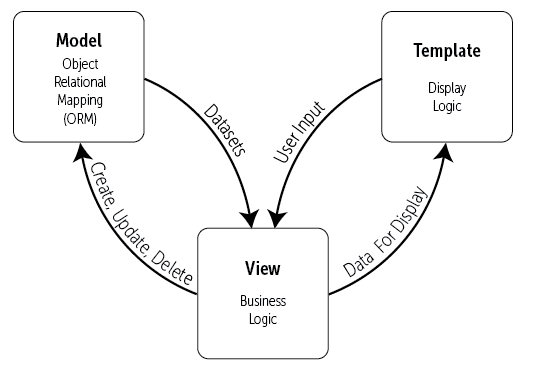
\includegraphics[width=1\textwidth]{../images/Django.png}
	\captionsetup{justification=raggedleft, font={it, footnotesize}}
	\captionsetup{justification=justified, font={up, footnotesize}}
	\caption{Django design architecture}
	\label{rys1}
\end{figure}
This design philosophy allows developers to - 
\begin{itemize}
	\item  Run servers separately for the database, media and applications.
	\newline
    
	\item  Easily have media served from a CDN (Content Delivery Network)
	\newline
    
	\item  Cache content at multiple scopes and levels
	\newline
    
	\item  For large web applications, it enables clustering and load-balancing in order to distribute the website across multiple servers
    
\end{itemize}
Web programming and web design are two very different ideas. For everything but the small prkects, the programming and design is not done by the same person, in many situations it is not even done by the same company. Django's template system makes it clear that Django programmers and websites must be able to work independent from each other. The profit is a plain text scripting language which makes use of tags to provide the presentation logic that decides what content needs to be displayed in the template.

DRY (Don't Repeat Yourself) is a term that often comes up, and it is one of Django's core principles. The DRY principle is evident in how Django makes use of template inheritance and helps reduce repetition and redundant code. Django comes with a large set of in-built tools that can be used out of the box without prior setup requirement. It provides some common, however complex processes in the form of wrappers. Some of these packages include administration, authorization, database specific features, session management, syndication, etc.
Django provides high security by disallowing code execution inside a webpage. This simple approach provides high security compared to other languages such as Javascript which can be executed within the browser and hence keeps the door open to various kind of vulnerabilities.



\subsection{.NET}
    
.NET Core is known to be a modular, cross-platform, general-purpose and open source implementation of the .NET Standard. It contains a huge number of APIs similar to the .NET Framework (but .NET Core is a smaller set) and incorporates runtime, architecture, compiler and tools components that support a variety of operating systems and chip targets. The implementation of .NET Core was mainly emphasized by the ASP.NET Core workloads but also by the need to have a more modern architecture of the framework. It can be used in many situations such as in device, cloud and embedded/IoT scenarios. \cite{dotnet}.
\newline
    
.NET Core is supported on Windows, macOS and Linux. However, on Linux, Microsoft mainly supports .NET Core that runs on Red Hat Enterprise Linux (RHEL) and other Debian distribution families. .NET Core currently only supports X64 CPUs although on Windows, X86 is also supported. Support for ARM64 and ARM32 are in progress.
\newline
    
Here are the main characteristics of .NET Core:
\newline
    
\begin{itemize}
  \item \textbf{Cross-platform} - .NET Core comes with key functionality to implement the application features needed by developers and reusability of code regardless of the target platform. The three three major operating systems that are supported are: Windows, Linux and macOS. Applications and libraries can be written without any need for modifications across supported operating systems.
  \newline
    
  \item \textbf{Open source} - .NET Core is one of the numerous projects under the ownership of the .NET Foundation and is accessible on GitHub. Being oper source, .NET Core promotes a more straightforward development process and advances a dynamic and engaged community.
  \newline
    
  \item \textbf{Flexible deployment} - There are two major mothods to deploy a .NET application: the deployment dependant on the framework or a self-contained deployment. With the former, only the application and any third-party libraries are installed and the application depends on a system version of .NET Core to be installed. With the latter however, the version of .NET Core used to compile the application is also deployed with the application along with third-party libraries and can run side-by-side with different versions \cite{dotnet}.
  \newline
    
  \item \textbf{Modular} - .NET Core is considered to have a modular architecture since it is released through NuGet package manager in smaller assembly packages. Rather than one large assembly that contains most of the core functionality, .NET Core is made available as smaller feature-centric packages. Thanks to this, developers are able to work in a more agile development model which allows them to optimize applications to include just the NuGet packages needed. The advantages of a smaller application surface area include tighter security, improved performance, reduced servicing, and low costs in a pay-for-what-you-use model \cite{dotnet}.
\end{itemize}
    
.NET Core is composed of the following parts:
\begin{itemize}
\item A .NET runtime environment, that provides a type system, a garbage collector, native interoperability, assembly loading and other services.
   
\item A set of libraries, which provide features like primitive data types, fundamental utilities and app composition types.
   
\item A set of development tools and language compilers that helps the base developer experience, available in the .NET Core SDK.

\item The 'dotnet' application host, that is used to launch .NET Core appilcations. It hosts the runtime, providing an assembly loading policy to launch the applications. It is also used to launch SDK tools.
\end{itemize}

\subsection{Database - PostgreSQL}
PostgreSQL is an object-relational database management system that emphasizes on the principles of extensibility and standards compliance. The primary function is to store data in a secure manner and return the data as response when requests are made to the database from software applications. It is able to handle high workloads that range from small single-machine applications to very large-scale applications for purposes such as data warehousing that have many concurrent users. 
PostgreSQL requires mininum maintenance because it is very stable. Therefore applications developed on PostgreSQL have low total cost of ownership compared to other database management systems.
\linebreak

Some of the important features of PostgreSQL are as follows -
\smallskip
\begin{itemize}
	\item User-defined types
	\smallskip
	\item Table inheritance
	\smallskip
	\item Sophisticated locking mechanism
	\smallskip
	\item Views, rules, subquery
	\smallskip
	\item Nested transactions
	\smallskip
	\item Asynchronous replication
	\smallskip
	\item Foreign key referential integrity
	\smallskip
	\item Multi version concurrency control	
\end{itemize}
PostgreSQL is compliant to standards. Its implementation of SQL conforms to ANSI-SQL:2008 standard. PostgreSQL supports all subqueries of SQL including subselects, it is also read-committed and serializes transaction isolation levels.
The data security and integrity features that come with postgreSQL are primary keys, foreign keys with cascading updates and deletes as well as restrictions, check constraints, not null constraints and unique constraints.
\newline

Some of the advantages of using PostgreSQL are - 
\begin{itemize}
	\item \textbf{Immunity to over-deployment}
	Over-deployment is a major problem in most proprietary database vendors such as Oracle SQL. But with PostgreSQL, since it has no associated licensing cost for using the software, there are no legal restrictions or compliances to follow.
	\smallskip
	\item \textbf{Extensible}
	The source code for PostgreSQL is open-source. If a database administrator needs to customise or extend PostgreSQL, they are free to do so and require minimum effort with no added costs.
	\item \textbf{Cross platform}
	PostgreSQL is available on all the major UNIX operating systems as well as Windows and macOS via the cygwin framework.
	\item \textbf{Low staffing and maintenance cost}
	PostgreSQL is designed to have minimum maintenance and tuning requirements as compared to other proprietary databases, while providing all the features, performance and stability.
\end{itemize}
\subsection{ApacheBench}
ApacheBench (ab) is a single-threaded command line computer program for measuring the performance of HTTP web servers. Originally designed to test the Apache HTTP Server, it is generic enough to test any web server.
The ab tool comes bundled with the standard Apache source distribution, and like the Apache web server itself, is free, open source software and distributed under the terms of the Apache License. \cite{ab}
Apachebench generates a flood of queries to the specified URL and returns a variety of metrics. These metrics can be used to compare the performance of various web technologies in our project. Some of the important metrics are requests/second, time per request, and transfer rate. The tool allows testers to load test a URL or server by replicating number of users and number of concurrent requests per second.

\subsection{JMeter}
JMeter is an Open Source testing software. It is written purely in Java application for the purpose of performance and load testing. JMeter covers a variety of categories of tests like functional, performance, stress, regression,  etc., and requires JDK 5 or higher to run. \cite{jmeter}
\newline
    
JMeter simulates a group of users sending requests to a server, and returns imformation that shows the performance/functionality of the target server/application via tables, graphs, etc.
\newline
    
%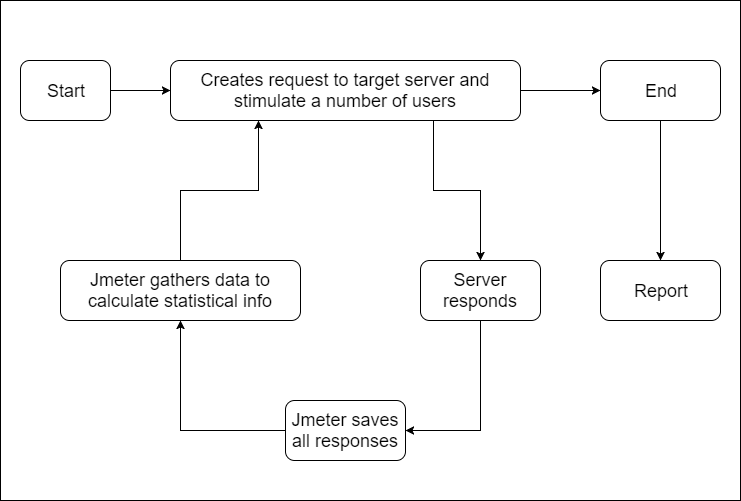
\includegraphics[width=150mm]{Jmeter.png} 
    
The protocols supported by JMeter are -

\begin{itemize}
	\item \textbf{Web} - HTTP, HTTPS sites 'web 1.0' web 2.0 (ajax, flex and flex-ws-amf)
  
	\item \textbf{Web Services} - SOAP / XML-RPC

	\item \textbf{Directory} - LDAP
   
	\item \textbf{Service} - POP3, IMAP, SMTP
  
	\item Database via JDBC drivers
    
	\item Messaging Oriented service via JMS
   
	\item FTP Service
\end{itemize}

\subsection*{Features}
\begin{itemize}
	\item Being an open source software, JMeter is freely available.
   
	\item Simple graphical user interface.
   
	\item JMeter is able to conduct performance tests for a variety of server types: Web - HTTP, HTTPS, Database via JDBC, LDAP, Mail - POP3, etc.
  
	\item It is independent of operating system. JMeter can be invoked by clicking on JMeter shell script on Linux/Unix OS. It can be invoked by starting the jmeter.bat file on the different versions of Windows.
    
	\item It supports full Swing and lightweight components.
   
	\item JMeter store its results and test plans in XML format. This means that users can generate a test plan using a text editor.
 
	\item Its multi-threading framework enables simultaneous sampling by many threads and concurrent sampling of different functions by separate thread groups.
   
	\item It is highly extensible.
   
	\item It can also be used to perform automated and functional testing of the applications.
    
\end{itemize}

\subsection{DigitalOcean}
DigitalOcean is an IaaS (Infrastructure as a Service) company that delivers fast and easy solutions for developers and bsuinesses to deploy their applications on the cloud. It accelerates software development so that the developers and programmers can spend more time working on the feature building and less tiem and focus on managing the infrastructure. 
\newline

DigitalOcean virtual servers (VPS) also known as "droplets" use KVM (Kernel-based Virtual Machine) as hypervisor and so they can be created in a variety of different sizes. DigitalOcean has their data center in eight different regions around the world, and provides 6 GNU/Linux distributions and dozens of on-click setup applications. DigitalOcean also offers an additional feature of load balancing on their cloud servers. They provide a scalable infrastructure for programmers to build applications with fast development times.
\newline

DigitalOcean's services are specifically created for all scales of applications, from individual based to enterprise based. They offer serveral different levels of cloud based hosting considering different requirements such as storage capacity, volume needs, and also billed either on a monthly or hourly basis. The more the features, will determite the amount of memory, disk space, transfer limit and core processors provided by the server in your chosen plan.
\newline

Setting up a DigitalOcean virtual server or "droplet" can be done in under a minute. With each droplet, the developer gets full root access to the server, with the ability to customize the server setup and choose the desired operating system.

All of DigitalsOcean's plans include the following - 
\begin{itemize}
	\item Solid state drives (SSD)
   
	\item Simple account control panel
   
	\item DNS management
   
	\item Global image transfer (gives the developers the ability to load droplets in different datacenters)
  
	\item Private networking (different droplets belonging to you can communicate with each other with no restrictions on bandwidth limits)  
\end{itemize}
\subsection*{Technology and Infrastructure}
DigitalOcean has set up its datacenters each in London, Singapore, San Francisco and three each in Amsterdam and New York. The datacenter in Singapore supports IPv6. Cloud servers are deployed using the KVM virtualization build on Intel's Hex-Core CPUs that have a RAID SSD storage and dedicated ECC RAM. However, the developer can use the control panel or DigitalOcean's name-spaced API to design their own. The control panel also provides a one-click install of common apps such as Linux distributions on the droplets, such as FreeBSD, CentOS, Ubuntu, Drupal or Wordpress.
Security is one of the most important concerns when it comes to web hosting, but it becomes even more important on cloud hosting. DigitalOcean restricts access to the most critical systems, so the technical staff does not have any access to backend hypervisors, so only the engineering team can access snapshots of the storage systems as well as backups. The datacenters are protected physically by security staff that are working round-the-clock. Biometric readers and two factor authentication are also provided as a safety measure. DigitalOcean promises a 99.99\% uptime, and offers credit if the downtime is below that level.

\subsection*{Features}
\begin{itemize}
	\item \textbf{Teams} - This features allows the developers to share resources and accounts between multiple teams and projects. By inviting teams members to streamline a lot of the manual work. The team members can have various roles such as some responsible for managing resources and billing across multiple sites or apps, provide an overview to make sure that all the team members are using the best practices for security, etc.
	\newline
    
	\item \textbf{Block Storage} - Whenever more storage is required, it is easy to extend additional storage to the droplets as per our requirement. The storage blocks are separate from the actual server droplet and have multiple copies that are spreat out throughout the network of servers to make sure that the data is protected in rare situations of hardware failure.
	\newline
    
	\item \textbf{Resilient Network} - By making use of Tier - 1 bandwidth, DigitalOcean's worldwide network is optimized so that it delivers data wherever it has to go, with high speed and high security. It is possible to instantly deploy by using load balancers which improve the reliability of the droplet server.
	\newline
    
	\item \textbf{Spaces} - In addition to block storage, DigitalOcean provides a cloud storage solutions called Spaces. It is used as a store for important data.
	\newline
    
	\item \textbf{One-click Installs} - When setting up a droplet, it is possible to imstall many different types of applications, scripts or CMS systems with just one click instead of logging in to the console and do it all from scratch.
	\newline
    
	
\end{itemize}

\end{document}
